\section{Results} \label{sec:results}

\subsection{The capacitor as a function of charge} \label{sec:results:exp1}

According to Section \ref{sec:theory}, the potential difference in the capacitor is linearly proportional to the charge stored on the capacitor. The experimental data (see Table \ref{tab:appendix:data:exp1}) was plotted and fed against the linear function $V(q) = Cq$ in Figure \ref{fig:results:exp1}. For each number of applied charges $q$, the mean voltage $V_C$ and the mean-squared-error $\Delta V_C$ were calculated using:
\begin{equation*}
    V_C := \left< V_C \right> = \frac{1}{5}\sum_{i=1}^{5} V_{C_i} \text{  and  } \Delta V_C := \frac{1}{5}\sqrt{ \sum_{i=1}^{5} (V_{C_i} - \left< V_C \right>)^2 }
\end{equation*}

Table \ref{tab:results:exp1} shows the resulting mean voltage values and uncertainties for each number of applied charges for two separations of $s_1 = 2(mm)$ and $s_2 = 4(mm)$.
\begin{table}[H]
    \centering
    \begin{minipage}{\textwidth}
        \centering
        \begin{tabular}{|c|cccccccccc|}
             \hline
             $q$               & 1 & 2 & 3 & 4 & 5 & 6 & 7 & 8 & 9 & 10 \\
             \hline
             $V_C, (V)$        & 0.7 & 1.7 & 2.6 & 3.3 & 3.9 & 4.7 & 5.2 & 5.7 & 6.3 & 6.6 \\
             $\Delta V_C, (V)$ & 0.2 & 0.2 & 0.3 & 0.6 & 0.4 & 0.8 & 0.9 & 1.0 & 1.3 & 1.4 \\ 
             \hline
        \end{tabular}
        \caption{$s_1 = 2(mm)$}
    \end{minipage}

    \vspace{0.5cm}
    
    \begin{minipage}{\textwidth}
        \centering
        \begin{tabular}{|c|cccccccccc|}
             \hline
             $q$               & 1 & 2 & 3 & 4 & 5 & 6 & 7 & 8 & 9 & 10 \\
             \hline
             $V_C, (V)$        & 3.2 & 5.8 & 8.1 & 10.3 & 12.6 & 15.0 & 17.1 & 17.6 & 19.8 & 21.8 \\
             $\Delta V_C, (V)$ & 0.4 & 0.9 & 0.6 & 1.8 & 2.0 & 2.1 & 1.8 & 3.7 & 3.6 & 4.1  \\ 
             \hline
        \end{tabular}
        \caption{$s_2 = 4(mm)$}
    \end{minipage}

    \caption{Mean voltage values and uncertainties}
    \label{tab:results:exp1}
\end{table}

\begin{figure}[H]
    \centering
    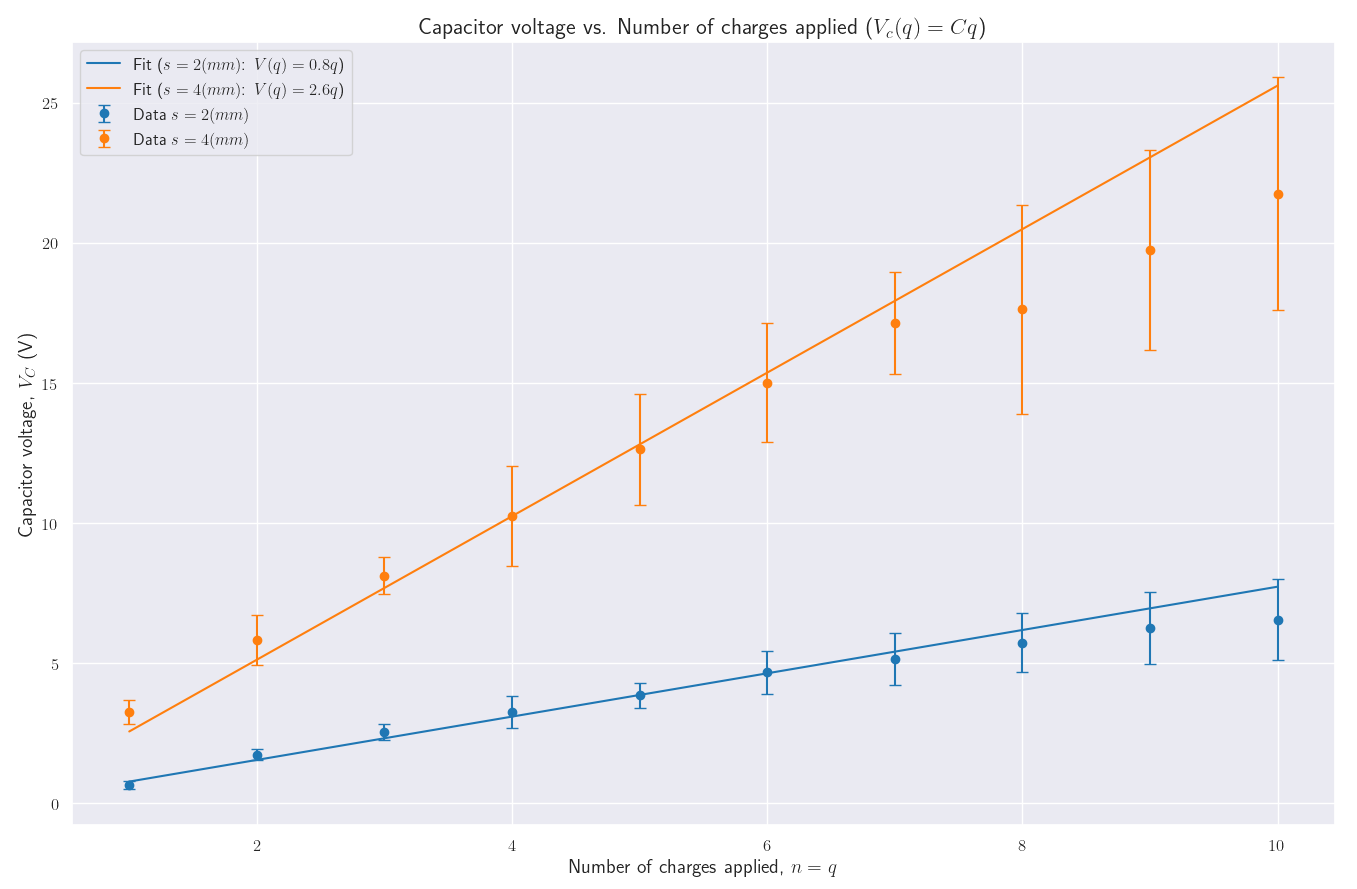
\includegraphics[width=\textwidth]{capacitors/img/capacitor_voltage_graph.png}
    \caption{The capacitor voltage as a function of the number of charges applied.}
    \label{fig:results:exp1}
\end{figure}

The graph is indeed linear with accumulating distortions as the number of applied charges $q$ increases. To fit data into the curve, the Levenberg-Marquardt algorithm \cite{scipy} was used which also returned the covariance matrix of the parameters. For $s_1 = 2(mm)$, $k = C_1 = 0.8 \pm 0.001$; whereas for $s_2 = 4(mm)$, $k = C_2 = 2.6 \pm 0.01$. The uncertainty in the best-fit functions is not displayed because only the trend is crucial.

\subsection{The distribution of charge on a surface} \label{sec:results:exp2}

In Section \ref{sec:theory}, it was discussed that the field in-between the capacitor plates is uniform and homogeneous. Therefore, the expected radial volume charge distribution $\rho$ was expected to be linear at first but to begin to deviate at the edges.

The raw data for this experiment can be found in Table \ref{tab:appendix:data:exp2} in Appendix \ref{appendix:data}. Since the distance from the center of the capacitor plate was measured by the human eye, its intrinsic error is estimated to be $\Delta r = 0.002 (m)$. This value is not shown on the $\rho$ graph and is not taken into account when calculating the best-fit function. For each distance $r$, the mean voltage $V$ and its uncertainty $\Delta V$ were calculated using\footnote{As discussed in Appendix \ref{appendix:data}, there are $11$ measurements each sampled $3$ times for the distribution of charge on a surface experiment.}:

\begin{equation*}
    V := \left< V \right> = \frac{1}{3}\sum_{i=1}^{3} V_i \text{  and  } \Delta V := \frac{1}{3}\sqrt{ \sum_{i=1}^{3} (V_i - \left< V \right> )^2 }
\end{equation*}

The resultant tabular data is shown in Table \ref{tab:results:exp2}, and plotted in the graph and the disk in Figure \ref{fig:results:exp2}.

\begin{table}[H]
    \centering
    \begin{tabular}{|c|ccccccccccc|}
        \hline
         $r, (m)$        & 0.00 & 0.01 & 0.02 & 0.03 & 0.04 & 0.05 & 0.06 & 0.07 & 0.08 & 0.09 & 0.10 \\
         $V, (V)$        & 3.2 & 3.2 & 3.0 & 3.3 & 3.2 & 3.2 & 3.7 & 4.1 & 4.5 & 5.8 & 6.5 \\
         $\Delta V, (V)$ & 0.2 & 0.2 & 0.4 & 0.2 & 0.3 & 0.2 & 0.2 & 0.1 & 0.05 & 0.2 & 0.1 \\
         \hline
    \end{tabular}
    \caption{Uncertainties and voltages for the distribution experiment.}
    \label{tab:results:exp2}
\end{table}

The best-fit curve was chosen to be the sigmoid function $V(r) = \frac{a}{1 + e^{-\frac{r + b}{d}}} + c$. The reason and further explanation on the abrupt jump in the surface charge distribution is further addressed in Section \ref{dis:exp2}. The best-fit algorithm \cite{scipy} gives the following parameters and uncertainties:

\begin{equation*}
    \begin{cases}
        a = -5.9 \pm 2.9, \\
        b = -0.1 \pm 0.01, \\
        c = 9.1 \pm 2.8, \\
        d = -0.01 \pm 0.005
    \end{cases}
\end{equation*}

\begin{figure}[H]
    \centering
    \includegraphics[width=0.75\linewidth]{capacitors/img/distribution_graph.png}
    \caption{The surface charge distribution as a function of radial d}
    \label{fig:results:exp2}
\end{figure}

\subsection{The potential difference as function of the plate distance at constant charge} \label{sec:results:exp3}

The following table shows the capacitor voltage $V$ against the separation of its plates. This table uses data shown in Appendix A Table\ref{tab:appendix:data:exp3}. The error $\Delta V$ was calculated using the standard deviation: $\sigma = \sqrt{\left<V^2\right> - \left<V\right>^2}$.

\begin{table}[H]
    \begin{minipage}{\textwidth}
    \centering
        \caption{The mean and calculated error of capacitor voltage, $V$, measured at different separations $x$}
        \label{tab:results:exp3.1}
            \begin{tabular}{|c|c|c|} \hline 
             x $\pm 0.05 cm$   & $\left< V\right>, (V)$ & $\Delta V, (V)$ \\ \hline  
             1   & 41 & $\pm1$ \\ \hline 
             2   & 50 & $\pm7$\\ \hline 
             3   & 51 & $\pm4 $ \\ \hline  
             4   & 55 & $\pm6 $ \\ \hline 
             5   & 57 & $\pm5 $\\ \hline 
             6   & 52 & $\pm7$\\ \hline 
             7   & 56 & $\pm3 $\\ \hline 
             8   & 54 & $\pm3$\\ \hline 
             9   & 60 & $\pm1$\\ \hline 
             10  & 55 & $\pm7$\\ \hline 
             11  & 59 & $\pm6$\\ \hline 
             12  & 58 & $\pm8$\\ \hline
            \end{tabular}
    \end{minipage}
\end{table}

The graph of the capacitor voltage as a function of separation is shown in Figure \ref{fig:results:exp3.1}.

\begin{figure}[H]
    \centering
    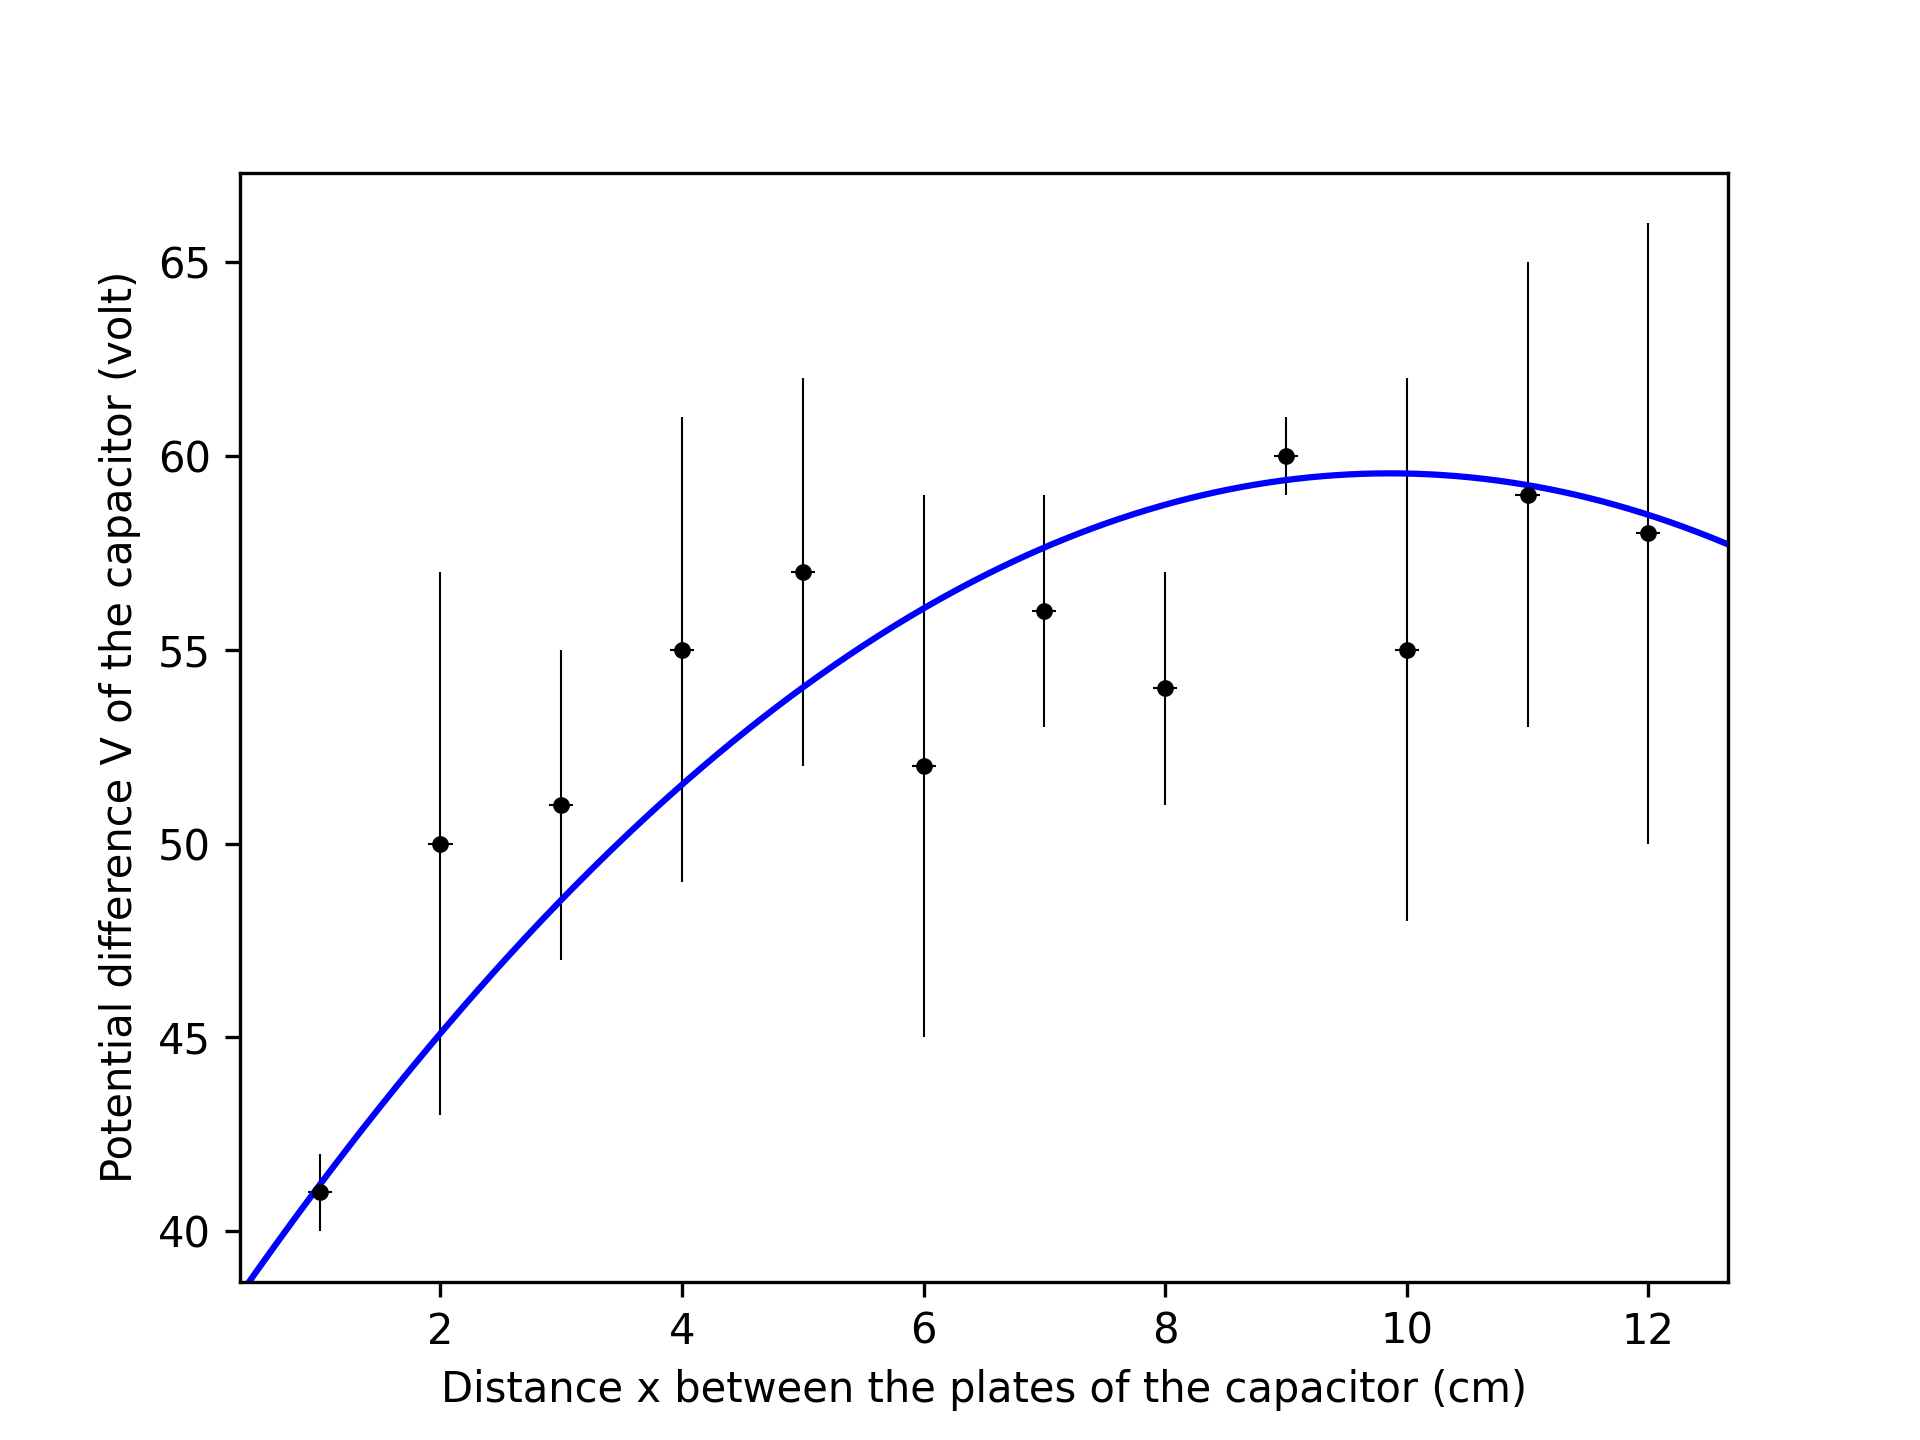
\includegraphics[width=\textwidth]{capacitors/img/Capacitor_distance_vs_V_graph.png}
    \caption{The potential difference as a function of the plate distance.}
    \label{fig:results:exp3.1}
\end{figure}

The relation between the separation $x$ between the plates of the capacitor and the potential is quadratic, as can be seen in Figure \ref{fig:results:exp3.1}. The quadratic expression of this relation is given by $ax^2+bx+c$ with parameters $a= -0.23 \pm 0.09$, $b= 17 \pm1 $, and $c=4.6 \pm 0.9$. 

In Figure \ref{fig:results:exp3.1}, the data in Table \ref{tab:results:exp3.1} is plotted: $\frac{1}{V}$ as a function of $\frac{1}{x}$. The error in $\frac{1}{V}$ is propagated using $Z = \frac{B}{A} \Rightarrow (\frac{\Delta Z}{Z})^2= (\frac{\Delta A}{A})^2 +(\frac{\Delta B}{B})^2$. In our case $B = 1$, and thus $\Delta (1/V) = \frac{\Delta V}{V^2}$. The resultant data is shown in Table \ref{tab:results:exp3.2} and Figure \ref{fig:results:exp3.2}.

\begin{table}[H]
    \begin{minipage}{\textwidth}
    \centering
        \caption{The mean and error margin of $\frac{1}{V}$ at intervals of $\frac{1}{x}$}
        \label{tab:results:exp3.2}
        \begin{tabular}{|c|c|c|} \hline 
        $\frac{1}{x}$       &  mean of$\frac{1}{V}$ & error in $\frac{1}{V}$ \\ \hline 
        1.00       & 0.0244 & $\pm$0.0005 \\ \hline 
        $0.50$      &0.020  & $\pm$0.003 \\ \hline 
        $0.33$      & 0.0120 & $\pm$0.002\\ \hline 
        $0.25$    & 0.018 &$\pm$0.002 \\ \hline 
        $0.20$    & 0.018 & $\pm$0.002 \\ \hline 
        $0.17$     & 0.019 & $\pm0.003$\\ \hline 
        $0.14$     & 0.018 & $\pm$0.001\\ \hline 
        $0.13$     & 0.019 & $\pm$0.001\\ \hline 
        $0.11$     & 0.0167& $\pm$0.0003\\ \hline 
        $0.10$     & 0.018 & $\pm$0.002\\ \hline 
        $0.09$     & 0.017 & $\pm$0.002\\ \hline 
        $0.08$     & 0.017 &$\pm$0.003 \\ \hline
        \end{tabular}
        \end{minipage}
\end{table}

\begin{figure}[H]
    \centering
    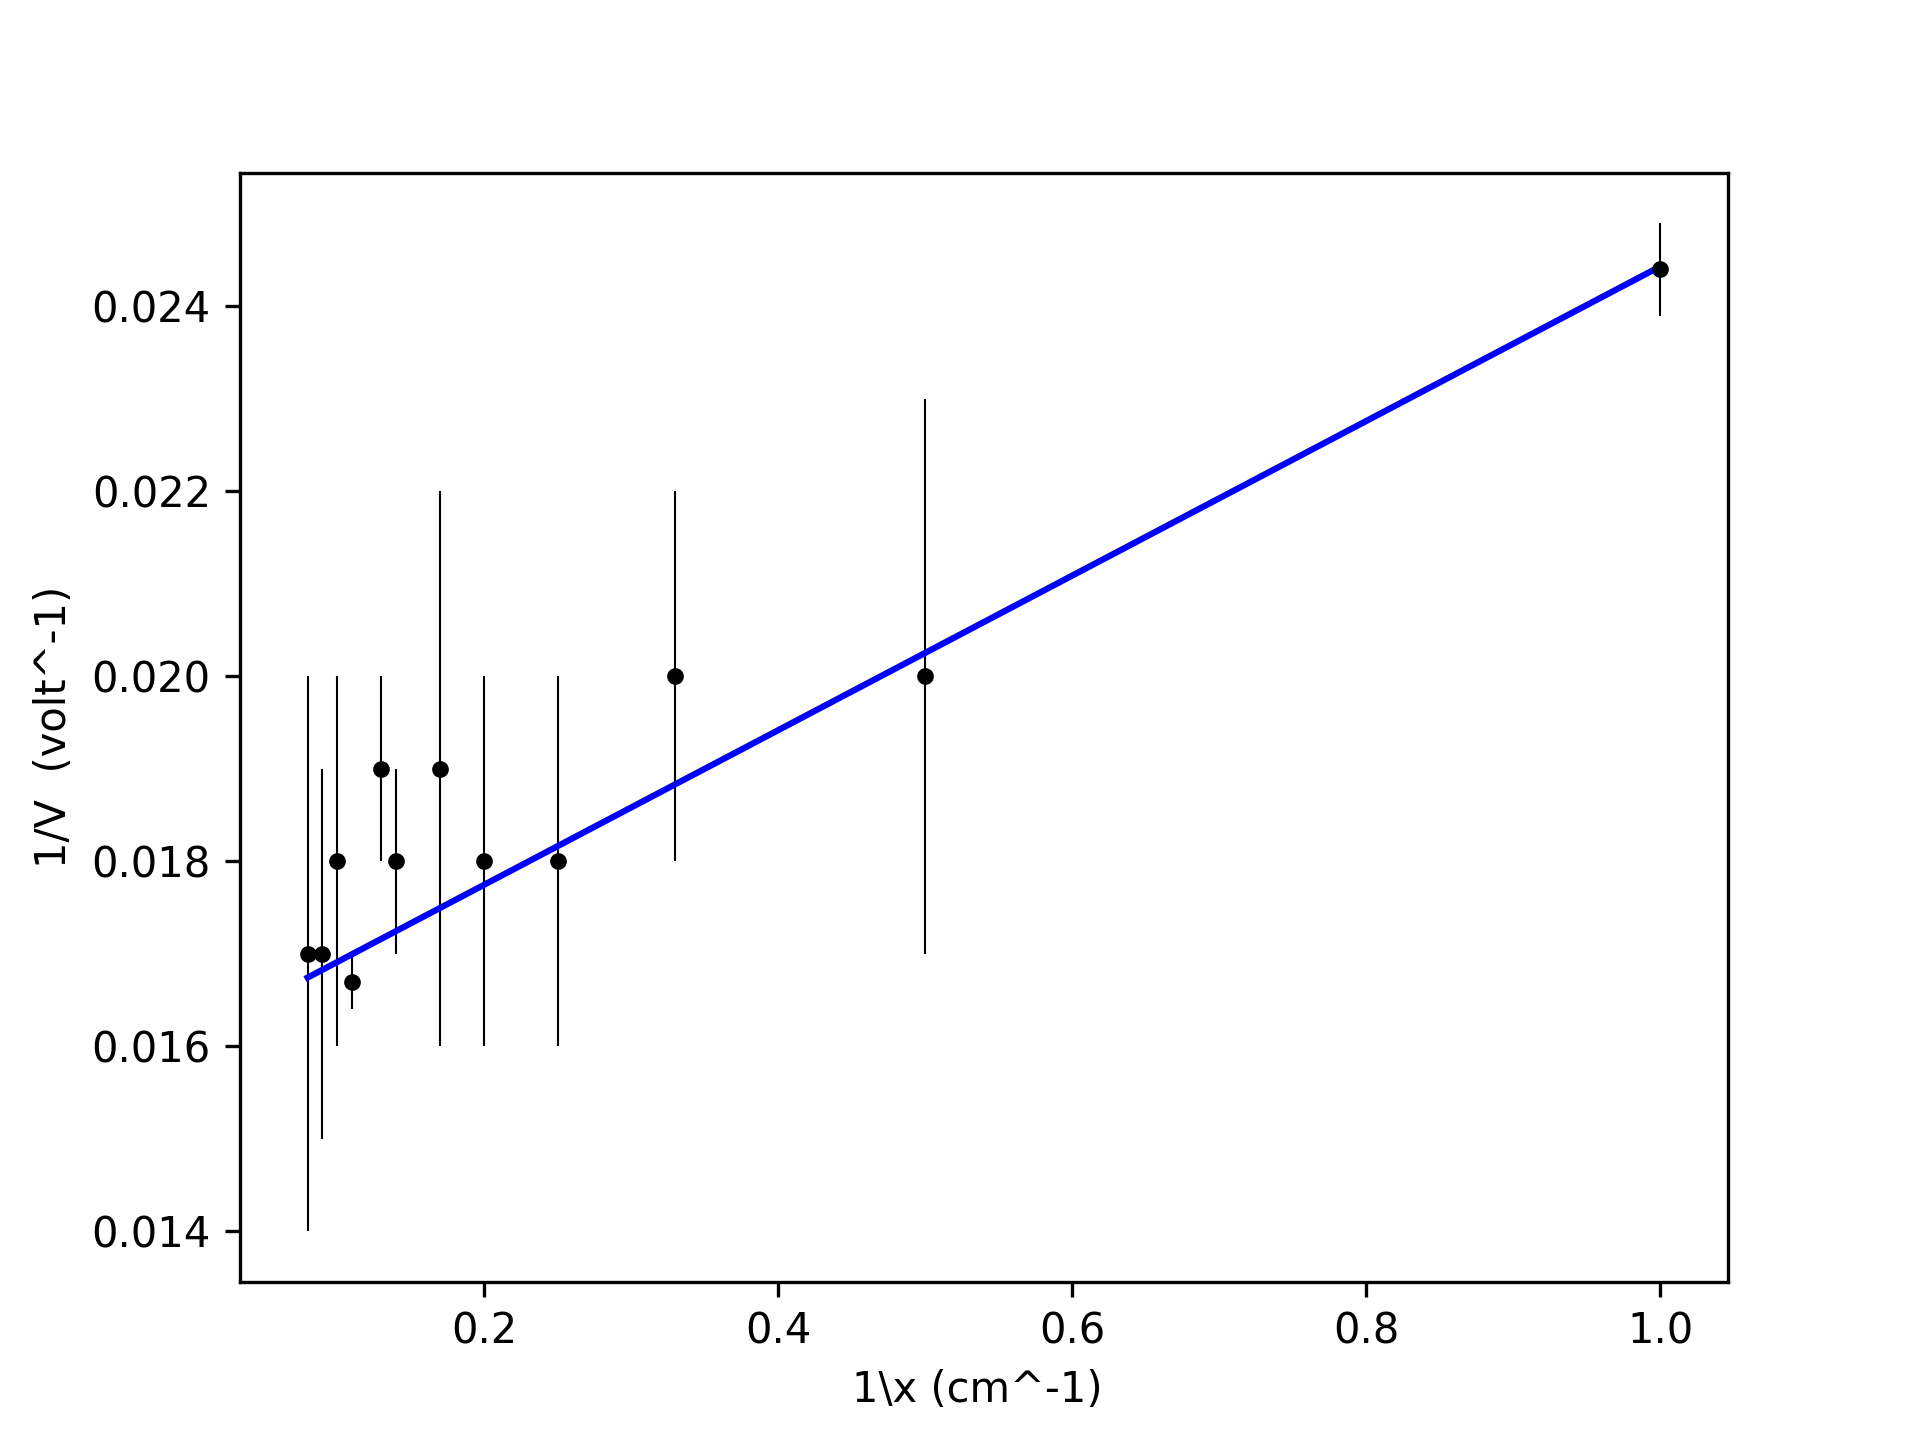
\includegraphics[width=\textwidth]{capacitors/img/Capacitor_1distance_vs_1V_graph.png}
    \caption{The 1/(potential difference) as a function of 1/(the plate distance).}
    \label{fig:results:exp3.2}
\end{figure}

The relation between $1/x$ and $1/V$ is linear. The linear expression of this relation is given by $ax+b$ with parameters of; $a= 0.084 \pm 0.005$ and $b= 0.0161 \pm 0.0003 $. 
